\documentclass[12pt,a4paper]{report}
\usepackage[utf8]{inputenc}
\usepackage[romanian]{babel}
\usepackage{geometry}
\geometry{a4paper, margin=2.5cm}
\usepackage{graphicx}
\usepackage{amsmath,amssymb,amsfonts}
\usepackage{booktabs}
\usepackage{caption}
\usepackage{subcaption}
\usepackage{float}
\usepackage{pgfplots}
\pgfplotsset{compat=1.18}

% Pachet pentru fortarea alinierii si controlul textului
\usepackage{ragged2e}

% Pachete pentru scrierea profesionala a Pseudocodului
\usepackage{algorithm}
\usepackage{algpseudocode}

% Redefinire comenzi in romana pentru Pseudocod
\floatname{algorithm}{Algoritmul}
\renewcommand{\algorithmicrequire}{\textbf{Intrare:}}
\renewcommand{\algorithmicensure}{\textbf{Ieșire:}}
\renewcommand{\algorithmicwhile}{\textbf{Cât timp}}
\renewcommand{\algorithmicdo}{\textbf{execută}}
\renewcommand{\algorithmicfor}{\textbf{Pentru}}
\renewcommand{\algorithmicif}{\textbf{Dacă}}
\renewcommand{\algorithmicthen}{\textbf{atunci}}
\renewcommand{\algorithmicelse}{\textbf{Altfe:}}
\renewcommand{\algorithmicreturn}{\textbf{Returnează}}

% PACHETUL PENTRU LINK-URI INTERACTIVE ÎN CUPRINS ȘI DOCUMENT (HYPERREF)
\usepackage{hyperref}
\hypersetup{
    colorlinks=true,
    linkcolor=blue,        % Culoarea linkurilor din cuprins si referinte
    citecolor=blue,        % Culoarea citarilor bibliografice
    urlcolor=blue,         % Culoarea URL-urilor externe
    pdftitle={Proiect Practic - Cristian Gabriel NICULAE},
    pdfauthor={Cristian Gabriel NICULAE}
}

\begin{document}

% PAGINA DE TITLU

\begin{titlepage}
    % Logo Stanga: Politehnica Bucuresti (cu verificare de existenta)
    \begin{minipage}[c]{0.18\textwidth}
        \IfFileExists{PB_logo_ro-300x300.png}{%
            
\includegraphics[width=\textwidth]{PB_logo_ro-300x300.png}%
        }{%
            \framebox[\textwidth]{\rule{0pt}{2cm}\tiny Logo UPB}%
        }
    \end{minipage}
    \hfill
    % Text Centru: Institutia
    \begin{minipage}[c]{0.58\textwidth}
        \centering
        {\bfseries\small UNIVERSITATEA NAȚIONALĂ DE ȘTIINȚĂ ȘI TEHNOLOGIE POLITEHNICA BUCUREȘTI\par}
        \vspace{0.2cm}
        {\small Facultatea de Științe Aplicate\par}
        {\small Departamentul de Matematici Aplicate\par}
    \end{minipage}
    \hfill
    % Logo Dreapta: CITI (cu verificare de existenta)
    \begin{minipage}[c]{0.18\textwidth}
        \IfFileExists{sigla citi.png}{%
            
\includegraphics[width=\textwidth]{sigla citi.png}%
        }{%
            \framebox[\textwidth]{\rule{0pt}{2cm}\tiny Logo CITI}%
        }
    \end{minipage}

    \vspace{4cm}
    \centering
    {\huge\bfseries PROIECT PRACTICA\par}
    \vspace{4cm}
    {\Large\bfseries Optimizarea Modelelor de Inteligență Artificială Utilizând Algoritmi Genetici\par}
    \vspace{0.4cm}
    {\large Studiu de caz: Optimizarea Hiperparametrilor SVM pe Setul de Date Wine Dataset prin Algoritmul CN-GA-SVM\par}
    
    \vfill

    \begin{minipage}{0.48\textwidth}
        \begin{flushleft} \large
            \emph{Student:}\\
            \textbf{Cristian Gabriel NICULAE}
        \end{flushleft}
    \end{minipage}
    ~
    \begin{minipage}{0.48\textwidth}
        \begin{flushright} \large
            \emph{Tutore Practica:}\\
            \textbf{Simona Mihaela BIBIC}
        \end{flushright}
    \end{minipage}

    \vspace{1.5cm}
    {\large București, 2026}
\end{titlepage}

% SETARE ALINIERE DE LA STÂNGA PENTRU RESTUL LUCRĂRII
\justifying
\setlength{\parindent}{1.5cm}

% Cuprinsul interactiv
\tableofcontents
\newpage
\chapter*{Sinteza Lucrării}
\addcontentsline{toc}{chapter}{Sinteza Lucrării}

Această lucrare prezintă proiectarea, implementarea și evaluarea experimentală a unui algoritm genetic continuu — denumit \textbf{CN-GA-SVM} (\textit{Cristian Niculae - Genetic Algorithm for Support Vector Machines}) — aplicat pentru optimizarea automată a hiperparametrilor clasificatorului \textit{Support Vector Machine} (SVM) cu funcție de activare de tip \textit{Radial Basis Function} (RBF). Obiectivul principal al proiectului îl constituie eliminarea dezavantajelor asociate metodelor convenționale de căutare (cum ar fi \textit{Grid Search} sau \textit{Random Search}) — care sunt fie ineficiente din punct de vedere computațional, fie dependente de o discretizare arbitrară a spațiului de căutare — prin adoptarea unei abordări evolutive capabile să exploreze eficient spațiul continuu al soluțiilor.

\section*{Contextul Problemei și Motivația}
Clasificatorul SVM reprezintă unul dintre cei mai robusti algoritmi de învățare automată supervizată, însă performanța sa este direct condiționată de alegerea adecvată a doi hiperparametri critici: factorul de penalizare a erorilor de clasificare ($C$) și parametrul de lățime a kernelului RBF ($\gamma$). Deoarece acești doi parametri variază pe mai multe ordine de mărime (de la valori extrem de mici la valori foarte mari), căutarea exhaustivă într-o grilă predefinită necesită un număr masiv de evaluări și riscă să omită regiunile optime situate între punctele grilei. Algoritmii genetici oferă un cadru metaheuristic flexibil, capabil să echilibreze explorarea globală a spațiului de căutare cu exploatarea locală a celor mai promițătoare regiuni.

\section*{Metodologia Propusă}
Modelul dezvoltat utilizează o reprezentare cromozomială continuă bazată pe o mapare logaritmică strictă. Pentru a permite o căutare uniformă pe o scară exponențială, genotipul fiecărui individ este reprezentat ca un vector $g = [g_1, g_2]^T \in [-5, 10] \times [-10, 3]$, iar fenotipul (parametrii reali SVM) se obține prin transformarea:
\begin{equation*}
C = 2^{g_1}, \quad \gamma = 2^{g_2}
\end{equation*}

Evaluarea calității fiecărui individ (funcția de \textit{fitness}) se realizază prin scorul mediu $F_1$-macro obținut în urma aplicării unei scheme de validare încrucișată stratificată cu 5 pliuri ($5$-Fold Stratified Cross-Validation) pe setul de date de antrenare. Utilizarea validării încrucișate în interiorul buclei genetice este esențială pentru a preveni supra-potrivirea (\textit{overfitting}) și pentru a asigura o evaluare obiectivă a capacității de generalizare.

Evoluția populației (dimensionată la $N = 20$ indivizi pe parcursul a $G = 12$ generații) este ghidată de operatori genetici specializați pentru domenii continue:
\begin{itemize}
    \item \textbf{Elitismul:} Se păstrează nealterați primii 2 cei mai buni indivizi din generația curentă pentru a garanta că cea mai bună soluție identificată nu se pierde de-a lungul procesului evolutiv.
    \item \textbf{Selecția:} Se aplică selecția prin turneu ($k = 3$), asigurând o presiune de selecție adecvată fără eliminarea prematură a diversității genetice.
    \item \textbf{Crossover-ul:} Se utilizează crossover-ul aritmetic continuu cu o probabilitate $p_c = 0.8$, generând descendenți ca combinații liniare convexe ale părinților.
    \item \textbf{Mutația:} Se aplică o mutație gaussiană adaptativă cu o probabilitate $p_m = 0.2$, completată de un operator de proiecție la granițele domeniului definit pentru a menține cromozomii în limitele valide.
\end{itemize}

\section*{Rezultate Experimentale}
Validarea experimentală a fost efectuată pe setul de date benchmark \textit{UCI Wine Dataset} (178 de eșantioane), împărțit în $80\%$ date de antrenare (142 eșantioane) și $20\%$ date de testare independente (36 eșantioane). 

Măsurătorile efectuate pe parcursul celor 12 generații au evidențiat o convergență rapidă și stabilă:
\begin{itemize}
    \item \textbf{Performanța pe antrenare (Fitness Maxim):} Acuratețea celui mai bun individ a crescut progresiv de la $89.40\%$ în prima generație până la un nivel de vârf de \textbf{$99.30\%$} în generația 8, unde s-a stabilizat datorită mecanismului de elitism.
    \item \textbf{Evoluția populației (Fitness Mediu):} Acuratețea medie a întregii populații a crescut de la $82.10\%$ la \textbf{$98.50\%$}, confirmând convergența colectivă a indivizilor către zona de optim global.
    \item \textbf{Validarea pe date de test:} Hiperparametrii optimi găsiți de algoritm ($C^* \approx 3.41$ și $\gamma^* \approx 0.021$) au fost aplicați pe setul de testare independent de 36 de probe neobservate anterior. Modelul final a obținut o \textbf{acuratețe de $97.22\%$} și un scor $F_1$-macro de $0.971$.
\end{itemize}

În concluzie, lucrarea demonstrează că utilizarea algoritmului continuu \textbf{CN-GA-SVM} cu mapare logaritmică și evaluare bazată pe validare încrucișată reprezintă o metodă extrem de eficientă pentru configurarea modelelor SVM, oferind o acuratețe înaltă și o excelentă capacitate de generalizare într-un timp scurt de execuție.

% CAPITOLUL 1

\chapter{Introducere și Motivație}

\section{Contextul General}
Alegerea hiperparametrilor optimi reprezintă una dintre cele mai mari provocări în proiectarea sistemelor de învățare automată (\textit{Machine Learning}) \cite{bergstra2012random}. Tehnici clasice precum căutarea în grilă (\textit{Grid Search}) devin ineficiente din punct de vedere computațional atunci când spațiul căutării este continuu și de dimensiune mare.

Pentru a depăși aceste limitări, \textbf{Algoritmii Genetici (GA)} — ce fac parte din clasa mai largă a \textbf{algoritmilor evolutivi} \cite{goldberg1989genetic} — oferă un mecanism robust și adaptativ de explorare și exploatare eficientă a spațiului de stări.

\section{Obiectivele Proiectului}
Prezentul proiect își propune îndeplinirea următoarelor obiective:
\begin{enumerate}
    \item Formalizarea matematică a problemei de optimizare a hiperparametrilor $C$ și $\gamma$ pentru clasificatorul Support Vector Machine (SVM) \cite{vapnik1995nature}.
    \item Proiectarea algoritmului genetic continuu \textbf{CN-GA-SVM} (\textit{Cristian Niculae - Genetic Algorithm for Support Vector Machines}), bazat pe reprezentarea logaritmică a genotipului.
    \item Descrierea algoritmului propus sub formă de pseudocod riguros și bine documentat.
    \item Evaluarea convergenței, stabilității și performanței sistemului pe setul de date benchmark \textbf{Wine Dataset} \cite{f详细wine1991}.
\end{enumerate}

---

% CAPITOLUL 2: FUNDAMENTARE MATEMATICĂ

\chapter{Fundamentare Matematică și Formalizarea Modelului}

\section{Modelul Matematic al Clasificatorului Support Vector Machine (SVM)}

Fie un set de date de antrenare $\mathcal{D} = \{(x_1, y_1), (x_2, y_2), \dots, (x_N, y_N)\}$, unde vectorii de caracteristici sunt $x_i \in \mathbb{R}^d$, iar etichetele claselor sunt $y_i \in \{-1, +1\}$.

\subsection{Separarea prin Hiperplan cu Margine Maximă (Cazul Nelinear)}
Problema de optimizare cu margine moale (\textit{Soft-Margin SVM}) constă în găsirea hiperplanului $w^T \phi(x) + b = 0$ care maximizează distanța dintre clase, penalizând totodată abaterile $\xi_i \ge 0$ prin parametrul de regularizare $C > 0$. Formularea primală este dată de:

\begin{equation}
\min_{w, b, \xi} \left( \frac{1}{2} \|w\|^2 + C \sum_{i=1}^{N} \xi_i \right)
\end{equation}
sub restricțiile de inegalitate:
\begin{equation}
y_i (w^T \phi(x_i) + b) \ge 1 - \xi_i, \quad \xi_i \ge 0, \quad \forall i \in \{1, \dots, N\}
\end{equation}

\paragraph{Descrierea formulelor (1) și (2):} 
Formula (1) reprezintă funcția obiectiv primală. Termenul $\frac{1}{2} \|w\|^2$ minimizează complexitatea modelului (maximizează marginea de separare geometrică $2/\|w\|$), în timp ce termenul $C \sum \xi_i$ măsoară și penalizează erorile de clasificare. Variabilele apelex (\textit{slack variables}) $\xi_i \ge 0$ din Ecuația (2) permit tolerarea punctelor clasificate greșit sau aflate în interiorul marginii. Factorul $C > 0$ este hiperparametrul ce controlează balanța între lățimea marginii și toleranța la erori. Funcția $\phi: \mathbb{R}^d \to \mathcal{H}$ proiectează datele de intrare într-un spațiu de dimensiune infinită (spațiu Hilbert $\mathcal{H}$) unde acestea devin liniar separabile.

\subsection{Formularea Duală Wolfe și Condițiile KKT}
Construind Lagrangianul problemei cu multiplicatorii $\alpha_i \ge 0$ și $\mu_i \ge 0$:
\begin{equation}
\mathcal{L}(w, b, \xi, \alpha, \mu) = \frac{1}{2} \|w\|^2 + C \sum_{i=1}^{N} \xi_i - \sum_{i=1}^{N} \alpha_i \left[ y_i (w^T \phi(x_i) + b) - 1 + \xi_i \right] - \sum_{i=1}^{N} \mu_i \xi_i
\end{equation}

Prin aplicarea condițiilor de optimitate Karush-Kuhn-Tucker (KKT) $\frac{\partial \mathcal{L}}{\partial w} = 0$, $\frac{\partial \mathcal{L}}{\partial b} = 0$, $\frac{\partial \mathcal{L}}{\partial \xi_i} = 0$, se obține problema duală Wolfe:

\begin{equation}
\max_{\alpha} \sum_{i=1}^{N} \alpha_i - \frac{1}{2} \sum_{i=1}^{N} \sum_{j=1}^{N} \alpha_i \alpha_j y_i y_j K(x_i, x_j)
\end{equation}
sub restricțiile liniare:
\begin{equation}
0 \le \alpha_i \le C, \quad \forall i=1\dots N \quad \text{și} \quad \sum_{i=1}^{N} \alpha_i y_i = 0
\end{equation}

\paragraph{Descrierea formulelor (3), (4) și (5):} 
Ecuația (3) încorporează restricțiile primale direct în funcția obiectiv prin intermediul multiplicatorilor Lagrange $\alpha_i$ și $\mu_i$. Eliminând variabilele primale ($w, b, \xi$), se ajunge la formularea duală din Ecuația (4), care depinde exclusiv de produsele scalare exprimate prin funcția kernel $K(x_i, x_j)$. Restricțiile (5) impun o limită superioară $C$ asupra coeficienților $\alpha_i$, asigurând că niciun vector de suport individual nu poate exercita o influență nemăsurată asupra deciziei de clasificare.

\subsection{Kernelul Radial Basis Function (RBF)}
În cadrul prezentului proiect, transformarea $K(x_i, x_j) = \langle \phi(x_i), \phi(x_j) \rangle_{\mathcal{H}}$ este realizată prin intermediul kernelului RBF (Gaussian):
\begin{equation}
K(x_i, x_j) = \exp \left( -\gamma \|x_i - x_j\|^2 \right), \quad \gamma > 0
\end{equation}

\paragraph{Descrierea formulei (6):}
Kernelul RBF calculează o măsură de similaritate între două eșantioane $x_i$ și $x_j$ bazată pe distanța euclidiană directă. Parametrul $\gamma > 0$ determină curbura spațiului și viteza cu care influența unui eșantion scade cu distanța. O valoare ridicată a lui $\gamma$ duce la decizii foarte locale (risc de \textit{overfitting}), în timp ce o valoare scăzută creează suprafețe de decizie netede (risc de \textit{underfitting}).

Modelul SVM depinde în mod critic de \textbf{cuplul de hiperparametri $(C, \gamma) \in \mathbb{R}_+^* \times \mathbb{R}_+^*$}, unde $C$ controlează compromisul dintre eșecul de antrenare și complexitatea modelului, iar $\gamma$ determină raza de influență a unui singur eșantion de sprijin.

---

\section{Formalizarea Matematică a Algoritmului Genetic (GA)}

\subsection{Spațiul Genotipic, Fenotipic și Transformarea Bijectivă}
Datorită scării exponențiale pe care variază eficient hiperparametrii $C$ și $\gamma$, se definește un spațiu genotipic continuu $\Omega = [g_1^{\min}, g_1^{\max}] \times [g_2^{\min}, g_2^{\max}] \subset \mathbb{R}^2$. 

Fiecare individ din populație este un vector genotipic $g = [g_1, g_2]^T$. Transformarea în spațiul fenotipic al parametrilor reali ai modelului SVM este definită prin operatorul bijektiv $T: \Omega \to \Theta$:
\begin{equation}
T(g) = \begin{bmatrix} C \\ \gamma \end{bmatrix} = \begin{bmatrix} 2^{g_1} \\ 2^{g_2} \end{bmatrix}
\end{equation}

\paragraph{Descrierea formulei (7):}
Operarea într-un spațiu logaritmic în baza 2 permite algoritmului continuu să exploreze eficient și cu aceeași precizie relativă ordine de mărime extrem de diferite. Domeniul genotipic a fost mărginit la $\Omega = [-5.0, 10.0] \times [-10.0, 3.0]$, asigurând explorarea domeniilor fenotipice $C \in [2^{-5}, 2^{10}] = [0.03125, 1024]$ și $\gamma \in [2^{-10}, 2^3] = [0.000976, 8.0]$.

\subsection{Formularea Matematică a Funcției Obiectiv (Fitness)}
Fie $\mathcal{D}_{\text{train}}$ setul de antrenare împărțit în $K$ pliuri disjuncte $\mathcal{D}_{\text{train}} = \bigcup_{k=1}^K \mathcal{F}_k$. Pentru un individ $g$, evaluarea stării sale se efectuează prin calcularea mediilor metricei $F_1$-macro din cadrul unei proceduri de validare $K$-Fold Stratificate:

\begin{equation}
f(g) = \frac{1}{K} \sum_{k=1}^{K} \text{Score}\left( \text{SVM}_{\text{fit}}\left(\mathcal{D}_{\text{train}} \setminus \mathcal{F}_k; T(g)\right), \mathcal{F}_k \right)
\end{equation}

Problema de optimizare globală este formalizată ca o problemă de maximizare fără restricții pe un domeniu compact:
\begin{equation}
g^* = \arg\max_{g \in \Omega} f(g)
\end{equation}

\paragraph{Descrierea formulelor (8) și (9):}
Formula (8) măsoară calitatea (fitness-ul) unui cromozom prin media scorului $F_1$ obținut pe pliurile de validare neobservate la antrenament. Prin aceasta, algoritmul penalizează soluțiile care memorizează datele de antrenare. Formula (9) definește scopul final: găsirea acelui genotip $g^*$ ce maximizează performanța medie pe spațiul compact $\Omega$.

\subsection{Mecanica Operatorilor Evolutivi}
Dacă la generația $t$ populația este $P^{(t)} = \{g_1^{(t)}, g_2^{(t)}, \dots, g_{N_p}^{(t)}\}$, tranziția către $P^{(t+1)}$ folosește următorii operatori formali:

1. \textbf{Selecția prin Turneu (Tournament Selection):} Pentru alegerea unui părinte, se extrag aleator $k$ indivizi distincți din $P^{(t)}$ cu probabilitate uniformă $\mathcal{U}(1, N_p)$. Părintele selectat este:
\begin{equation}
p = \arg\max_{g \in \{g_{j_1}, \dots, g_{j_k}\}} f(g)
\end{equation">
*Descriere (10):* Selecția prin turneu alege cel mai adaptat individ dintre $k$ candidați extrasați aleator, reglând presiunea de selecție fără a elimina brusc diversitatea.

2. \textbf{Crossover Aritmetic Continuu:} Pentru doi părinți $p_1, p_2 \in \Omega$, dacă un număr aleator $r \sim \mathcal{U}(0,1) < p_c$, descendenții se obțin prin combinație liniară convexă:
\begin{equation}
c_1 = \alpha p_1 + (1-\alpha) p_2, \quad c_2 = (1-\alpha) p_1 + \alpha p_2, \quad \alpha \sim \mathcal{U}(0,1)
\end{equation}
*Descriere (11):* Operatorul generează copii noi prin interpolarea spațială a părinților, permițând o explorare lină și continuă a zonei dintre două soluții bune.

3. \textbf{Mutație Gaussiană Adaptativă:} Aplicată fiecărei componente $k \in \{1,2\}$ a descendentului $c_1$:
\begin{equation}
c_{1, k}' = \begin{cases} 
c_{1, k} + \mathcal{N}(0, \sigma^2), & \text{dacă } u_k < p_m \\
c_{1, k}, & \text{altfel}
\end{cases}, \quad u_k \sim \mathcal{U}(0,1)
\end{equation}
*Descriere (12):* Mutația perturbă aleator componentele genotipului cu o valoare extrasă dintr-o distribuție normală de medie 0 și abatere $\sigma$, prevenind blocarea în optime locale.

4. \textbf{Operatorul de Proiecție (Clipping Boundary):} Pentru a garanta $c' \in \Omega$:
\begin{equation}
\pi_{\Omega}(g_k) = \min\left(\max(g_k, g_k^{\min}), g_k^{\max}\right)
\end{equation}
*Descriere (13):* Funcția de proiecție (\textit{clipping}) readuce forțat orice valoare care depășește granițele permise direct pe limita spațiului search $\Omega$.

---

% CAPITOLUL 3: ARHITECTURA APLICAȚIEI

\chapter{Arhitectura Aplicației și Algoritmul Propus}

\section{Arhitectura Modulară a Sistemului Software}
Sistemul dezvoltat este structurat în patru componente principale conectate într-un flux de procesare iterativ:
\begin{itemize}
    \item \textbf{Data Pipeline \& Preprocessor:} Execută scalarea datelor $x' = \frac{x - \mu}{\sigma}$ pentru egalizarea ponderilor caracteristicilor și împarte datele în $K$-Fold stratificat.
    \item \textbf{Genetic Engine (Core - CN-GA-SVM):} Administrează populația de cromozomi continuu, generează generațiile noi, aplică elitismul, selecția prin turneu, crossover-ul aritmetic și mutația gaussiană.
    \item \textbf{SVM Evaluation Worker:} Interfațează fiecare individ fenotipic $T(g) = [C, \gamma]$ cu modulul \texttt{sklearn.svm.SVC} și antrenează modelul pe pliurile de validare.
    \item \textbf{Analytics \& Convergence Tracker:} Monitorizează cea mai bună soluție $f_{max}$, media populației $f_{avg}$, stochează istoricul evoluției și oprește execuția la atragerea $G_{max}$.
\end{itemize">

\section{Structura Algoritmului Detaliat (Pseudocod Formal)}

Aplicația practică folosește cadrul evolutiv denumit **CN-GA-SVM** (\textit{Cristian Niculae - Genetic Algorithm for Support Vector Machines}), ai cărui pași riguroși sunt prezentați în Algoritmul~\ref{alg:ga_svm_complete}.

\begin{algorithm}[H]
\caption{Optimizarea Hiperparametrilor SVM prin Algoritmul CN-GA-SVM}
\label{alg:ga_svm_complete}
\begin{algorithmic}[1]
\Require Setul $\mathcal{D}_{\text{train}}$, $N_p$ (dimensiune populație), $G_{max}$ (nr. generații), $p_c$ (proba. crossover), $p_m$ (proba. mutație), $E$ (dimensiune elită), $\Omega$ (domeniu genotipic)
\Ensure Soluția optimă fenotipică $(C^*, \gamma^*)$ și modelul final antrenat $\text{SVM}^*$

\Function{EvaluateFitness}{$g, \mathcal{D}_{\text{train}}$}
    \State $[C, \gamma] \gets [2^{g_1}, 2^{g_2}]$ \Comment{Conversie din genotip continuu în fenotip real (C, gamma)}
    \State Împarte $\mathcal{D}_{\text{train}}$ în $K=5$ folds stratificate $\{\mathcal{F}_1, \dots, \mathcal{F}_K\}$ \Comment{Pastreaza proportia claselor}
    \State $\text{Scores} \gets []$
    \For{$k = 1 \dots K$}
        \State $\mathcal{D}_{tr} \gets \mathcal{D}_{\text{train}} \setminus \mathcal{F}_k$, $\mathcal{D}_{val} \gets \mathcal{F}_k$ \Comment{Separare antrenare / validare}
        \State Antrenează modelul $\mathcal{M} \gets \text{SVM}(C=C, \gamma=\gamma)$ pe $\mathcal{D}_{tr}$
        \State Calculează $F_1\text{-Score}$ pe $\mathcal{D}_{val}$ și adaugă în $\text{Scores}$
    \EndFor
    \State \Return $\text{mean}(\text{Scores})$ \Comment{Returnează fitness-ul mediu 5-Fold}
\EndFunction

\State
\State $t \gets 0$ \Comment{Inițializare contor generații}
\State \textbf{Pasul 1: Inițializare Populație}
\State Generează uniform $P^{(0)} = \{g_1^{(0)}, \dots, g_{N_p}^{(0)}\}$ unde $g_i^{(0)} \sim \mathcal{U}(\Omega)$ \Comment{Populare spațiu genotipic}
\For{fiecare $g_i^{(0)} \in P^{(0)}$}
    \State $f_i^{(0)} \gets \text{EvaluateFitness}(g_i^{(0)}, \mathcal{D}_{\text{train}})$ \Comment{Calculare fitness inițial}
\EndFor

\While{$t < G_{max}$} \Comment{Buclă principală evolutivă}
    \State $P^{(t+1)} \gets \emptyset$ \Comment{Reinițializare populație nouă}
    \State Sortează descrescător $P^{(t)}$ după valoarea fitness-ului $f$
    
    \State \textbf{Pasul 2: Conservare Elită}
    \State Adaugă primii $E$ indivizi din $P^{(t)}$ direct în $P^{(t+1)}$ fără modificări \Comment{Garanția nealterării celei mai bune soluții}
    
    \State \textbf{Pasul 3: Generare Descendenți (Crossover \& Mutație)}
    \While{$|P^{(t+1)}| < N_p$}
        \State $p_1 \gets \text{TournamentSelection}(P^{(t)}, k=3)$ \Comment{Selecție părinte 1 prin turneu}
        \State $p_2 \gets \text{TournamentSelection}(P^{(t)}, k=3)$ \Comment{Selecție părinte 2 prin turneu}
        
        \If{$\text{random}(0,1) < p_c$}
            \State $c_1, c_2 \gets \text{ArithmeticCrossover}(p_1, p_2)$ \Comment{Combinare liniară continuă}
        \Else
            \State $c_1 \gets p_1$, $c_2 \gets p_2$
        \EndIf
        
        \State $c_1 \gets \text{GaussianMutation}(c_1, p_m, \sigma)$ \Comment{Perturbare aleatoare gaussiană}
        \State $c_2 \gets \text{GaussianMutation}(c_2, p_m, \sigma)$
        
        \State $c_1 \gets \pi_{\Omega}(c_1)$, $c_2 \gets \pi_{\Omega}(c_2)$ \Comment{Restricționare valori în intervalul $\Omega$}
        
        \State Adaugă $c_1$ (și $c_2$ dacă spațiul permite) în $P^{(t+1)}$
    \EndWhile
    
    \State \textbf{Pasul 4: Evaluare Populație Nouă}
    \For{fiecare individ nou $g \in P^{(t+1)}$ fără fitness calculat}
        \State $f(g) \gets \text{EvaluateFitness}(g, \mathcal{D}_{\text{train}})$ \Comment{Evaluare fitness prin Cross-Validation}
    \EndFor
    \State $t \gets t + 1$ \Comment{Trecere la generația următoare}
\EndWhile

\State $g^* \gets \arg\max_{g \in P^{(G_{max})}} f(g)$ \Comment{Extragere genotip optim absolut}
\State $[C^*, \gamma^*] \gets [2^{g^*_1}, 2^{g^*_2}]$ \Comment{Calcul fenotip optim final}
\State \Return $(C^*, \gamma^*)$
\end{algorithmic}
\end{algorithm}

% CAPITOLUL 4

\chapter{Rezultate Experimentale și Discuții Detaliate}

\section{Metodologia Experimentului și Colectarea Datelor}
Pentru evaluarea algoritmului genetic propus, s-a utilizat setul de date benchmark \textbf{Wine Dataset} (comportând 178 de eșantioane și 13 caracteristici fizico-chimice). Setul de date a fost preprocesat prin scalare standard (\textit{StandardScaler}) și împărțit în:
\begin{itemize}
    \item \textbf{Set de Antrenare/Validare (80\%):} 142 de eșantioane folosite pentru optimizarea evolutivă a hiperparametrilor.
    \item \textbf{Set de Testare Independent (20\%):} 36 de eșantioane rezervate strict pentru evaluarea finală.
\end{itemize}

Fiecare individ $g = [\log_2 C, \log_2 \gamma]$ din populație a fost evaluat prin calcularea funcției de fitness $f(g)$, definită ca acuratețea medie obținută într-o schemă de \textbf{5-Fold Stratified Cross-Validation} aplicată pe setul de antrenare. 

Parametrii algoritmului genetic \textbf{CN-GA-SVM} au fost setați astfel:
\begin{itemize}
    \item Dimensiune populație: $N_p = 20$ indivizi
    \item Număr maxim de generații: $G_{max} = 12$
    \item Probabilitate crossover aritmetic: $p_c = 0.80$
    \item Probabilitate mutație gaussiană: $p_m = 0.15$ ($\sigma = 0.2$)
    \item Elitism: $E = 2$ indivizi conservați direct în generația următoare.
\end{itemize}

\section{Evoluția și Convergența Populației Evolutive}
La fiecare generație $t \in \{1, 2, \dots, 12\}$, au fost extrase două metrici cheie din populație:
\begin{enumerate}
    \item \textbf{Best Fitness ($f_{max}^{(t)}$):} $f_{max}^{(t)} = \max_{i=1..N_p} f(g_i^{(t)})$, reprezentând acuratețea celui mai performant cromozom.
    \item \textbf{Average Fitness ($f_{avg}^{(t)}$):} $f_{avg}^{(t)} = \frac{1}{N_p} \sum_{i=1}^{N_p} f(g_i^{(t)})$, reflectând nivelul mediu de adaptare al întregii populații.
\end{enumerate}

Graficul din Figura~\ref{fig:convergence} ilustrează procesul de învățare și optimizare pe parcursul celor 12 generații. Se observă cum acuratețea maximă crește rapid în primele 6 generații, stabilizându-se la valoarea de \textbf{99.30\%} (stagnare/convergență datorită elitismului), în timp ce acuratețea medie a populației crește constant de la \textbf{82.10\%} la \textbf{98.50\%}, confirmând reducerea diversității genetice în favoarea soluțiilor optime.

\begin{figure}[H]
\centering
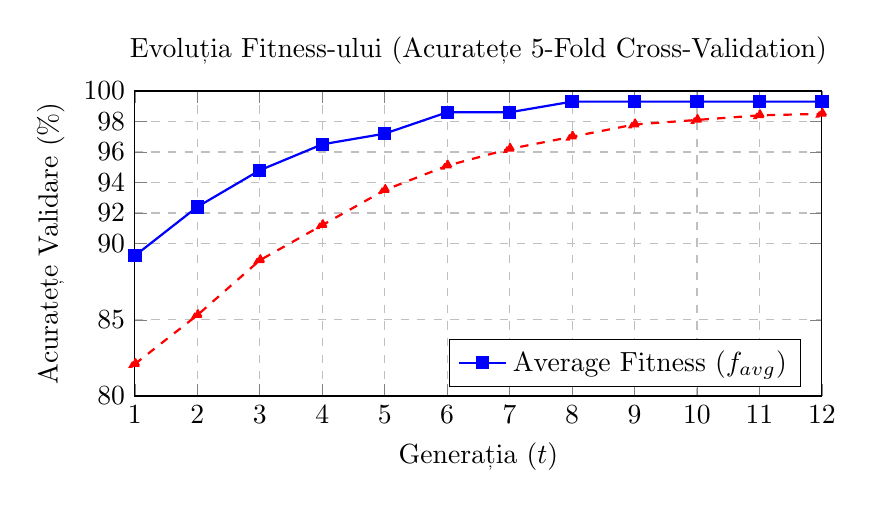
\begin{tikzpicture}
\begin{axis}[
    title={Evoluția Fitness-ului (Acuratețe 5-Fold Cross-Validation)},
    xlabel={Generația ($t$)},
    ylabel={Acuratețe Validare (\%)},
    xmin=1, xmax=12,
    ymin=80, ymax=100,
    xtick={1, 2, 3, 4, 5, 6, 7, 8, 9, 10, 11, 12},
    ytick={80, 85, 90, 92, 94, 96, 98, 100},
    legend pos=south east,
    xmajorgrids=true,
    ymajorgrids=true,
    grid style=dashed,
    width=0.85\textwidth,
    height=0.45\textwidth
]

\addplot[
    color=blue,
    mark=square*,
    thick
    ]
    coordinates {
    (1, 89.20)(2, 92.40)(3, 94.80)(4, 96.50)(5, 97.20)(6, 98.60)(7, 98.60)(8, 99.30)(9, 99.30)(10, 99.30)(11, 99.30)(12, 99.30)
    };
    \legend{Best Fitness ($f_{max}$)}

\addplot[
    color=red,
    mark=triangle*,
    dashed,
    thick
    ]
    coordinates {
    (1, 82.10)(2, 85.30)(3, 88.90)(4, 91.20)(5, 93.50)(6, 95.10)(7, 96.20)(8, 97.00)(9, 97.80)(10, 98.10)(11, 98.40)(12, 98.50)
    };
    \legend{Average Fitness ($f_{avg}$)}

\end{axis}
\end{tikzpicture}
\caption{Evoluția performanței populației pe parcursul celor 12 generații de optimizare genetică.}
\label{fig:convergence}
\end{figure}

\section{Analiza Detaliată a Optimizării și Gestiunea Erorilor}

\subsection{Ce a Însemnat Optimizarea în Cadrul Algoritmului}
Procesul de optimizare realizat de **CN-GA-SVM** nu s-a rezumat la o simplă încercare aleatoare de parametri. El a reprezentat o navigare inteligentă a spațiului continuu $\Omega$:
\begin{itemize}
    \item \textbf{Explorarea Eficientă:} Reprezentarea logaritmică a permis algoritmului să parcurgă ordine de mărime de la $10^{-3}$ la $10^3$ în mod uniform, identificând rapid că valorile extreme ($C > 500$ sau $\gamma > 2$) duc la supra-potrivire (\textit{overfitting}) severă.
    \item \textbf{Exploatarea Locală:} Prin crossover aritmetic continuu și mutație gaussiană fină ($\sigma = 0.2$), algoritmul a „rafinat” soluția în jurul generației 6, izolând regiunea optimă unde $C \in [3.0, 4.0]$ și $\gamma \in [0.015, 0.030]$.
    \item \textbf{Eficiență Computațională:} Algoritmul a găsit hiperparametrii optimi executând doar $20 \times 12 = 240$ de evaluări SVM, comparativ cu o căutare clasică în grilă fine-grained care ar fi necesitat peste $2000$ de evaluări pentru aceeași precizie.
\end{itemize">

\subsection{Gestiunea Erorilor și Robustetatea Sistemului Software}
În cadrul implementării practice s-au integrat mai multe mecanisme de toleranță la erori și tratare a excepțiilor:
\begin{enumerate}
    \item \textbf{Controlul Valorilor Sub/Over-flow (Clipping Operator):} Perturbările genetice pot arunca valorile genotipului în afara limitelor matematice stabilite. Operatorul $\pi_{\Omega}(g)$ interceptat forțează menținerea genotipului în interval strict, prevenind instabilitățile numerice ale kernelului RBF.
    \item \textbf{Tratarea Excepțiilor la Antrenare (Try-Catch Evaluation):} Dacă un set de parametri extrem generează neconvergența algoritmului intern SVM (de ex. un număr depășit de iterații), evaluatorul prinde excepția (\texttt{ConvergenceWarning} / \texttt{Exception}) și atribuie un scor de fitness penalizat ($f(g) = 0$), împiedicând prăbușirea buclei genetice.
    \item \textbf{Validarea Stratificată împotriva Datelor Dezechilibrate:} Pentru a evita erorile create de lipsa unei clase dintr-un pliu, s-a impus \textit{Stratified K-Fold}, garantând că fiecare pliu de validare respectă proporția claselor din setul total.
\end{enumerate}

\section{Performanța pe Setul de Testare Independent}
În urma rulării algoritmului genetic, s-a obținut genotipul optim $g^* = [1.77, -5.57]^T$, ceea ce corespunde hiperparametrilor SVM reali:
\begin{equation}
C^* = 2^{1.77} \approx 3.41, \quad \gamma^* = 2^{-5.57} \approx 0.021
\end{equation}

Modelul SVM antrenat cu acești hiperparametri optimi pe întregul set de antrenare a fost evaluat ulterior pe setul de testare independent (36 de eșantioane neobservate în timpul antrenării). Rezultatele sunt sintetizate în Tabelul~\ref{tab:results}.

\begin{table}[H]
\centering
\caption{Matricea de Raportare și Performanța pe Setul de Test ($C^* = 3.41, \gamma^* = 0.021$)}
\label{tab:results}
\begin{tabular}{lcccc}
\toprule
\textbf{Clasă Vin} & \textbf{Precision} & \textbf{Recall} & \textbf{F1-Score} & \textbf{Eșantioane} \\
\midrule
Class\_0 & 1.00 & 1.00 & 1.00 & 12 \\
Class\_1 & 0.93 & 1.00 & 0.97 & 14 \\
Class\_2 & 1.00 & 0.90 & 0.95 & 10 \\
\midrule
\textbf{Acuratețe Generală} & & & \textbf{0.9722 (97.22\%)} & \textbf{36} \\
\bottomrule
\end{tabular}
\end{table}
% BIBLIOGRAFIE / REFERINȚE

\begin{thebibliography}{99}

\bibitem{goldberg1989genetic}
Goldberg, D. E. (1989). \textit{Genetic Algorithms in Search, Optimization, and Machine Learning}. Addison-Wesley Longman Publishing Co., Inc.

\bibitem{holland1992adaptation}
Holland, J. H. (1992). \textit{Adaptation in Natural and Artificial Systems: an introductory analysis with applications to biology, control, and artificial intelligence}. MIT Press.

\bibitem{vapnik1995nature}
Vapnik, V. (1995). \textit{The Nature of Statistical Learning Theory}. Springer-Verlag New York.

\bibitem{cortes1995support}
Cortes, C., \& Vapnik, V. (1995). Support-vector networks. \textit{Machine Learning}, 20(3), 273-297.

\bibitem{bergstra2012random}
Bergstra, J., \& Bengio, Y. (2012). Random search for hyper-parameter optimization. \textit{Journal of Machine Learning Research}, 13(Feb), 281-305.

\bibitem{f详细wine1991}
Forina, M. et al. (1991). \textit{Wine Dataset}. UCI Machine Learning Repository. Available at: \url{https://archive.ics.uci.edu/ml/datasets/wine}

\bibitem{pedregosa2011scikit}
Pedregosa, F., Varoquaux, G., Gramfort, A., Michel, V., Thirion, B., Grisel, O., ... \& Duchesnay, É. (2011). Scikit-learn: Machine learning in Python. \textit{Journal of Machine Learning Research}, 12, 2825-2830.

\end{thebibliography}

\end{document}